
\documentclass[12pt]{article}
%\usepackage[finnish]{babel}
\usepackage[T1]{fontenc}
\usepackage[utf8]{inputenc}
\usepackage{amssymb}
\usepackage{amsmath}
\usepackage{graphicx}
\usepackage{hyperref}
\newcommand{\pat}{\partial}
\newcommand{\be}{\begin{equation}}
\newcommand{\ee}{\end{equation}}
\newcommand{\bea}{\begin{eqnarray}}
\newcommand{\eea}{\end{eqnarray}}
\newcommand{\abf}{{\bf a}}
\newcommand{\Zcal}{{\cal Z}_{12}}
\newcommand{\zcal}{z_{12}}
\newcommand{\Acal}{{\cal A}}
\newcommand{\Fcal}{{\cal F}}
\newcommand{\Ucal}{{\cal U}}
\newcommand{\Vcal}{{\cal V}}
\newcommand{\Ocal}{{\cal O}}
\newcommand{\Rcal}{{\cal R}}
\newcommand{\Scal}{{\cal S}}
\newcommand{\Lcal}{{\cal L}}
\newcommand{\Hcal}{{\cal H}}
\newcommand{\hsf}{{\sf h}}
\newcommand{\half}{\frac{1}{2}}
\newcommand{\Xbar}{\bar{X}}
\newcommand{\xibar}{\bar{\xi }}
\newcommand{\barh}{\bar{h}}
\newcommand{\Ubar}{\bar{\cal U}}
\newcommand{\Vbar}{\bar{\cal V}}
\newcommand{\Fbar}{\bar{F}}
\newcommand{\zbar}{\bar{z}}
\newcommand{\wbar}{\bar{w}}
\newcommand{\zbarhat}{\hat{\bar{z}}}
\newcommand{\wbarhat}{\hat{\bar{w}}}
\newcommand{\wbartilde}{\tilde{\bar{w}}}
\newcommand{\barone}{\bar{1}}
\newcommand{\bartwo}{\bar{2}}
\newcommand{\nbyn}{N \times N}
\newcommand{\repres}{\leftrightarrow}
\newcommand{\Tr}{{\rm Tr}}
\newcommand{\tr}{{\rm tr}}
\newcommand{\ninfty}{N \rightarrow \infty}
\newcommand{\unitk}{{\bf 1}_k}
\newcommand{\unitm}{{\bf 1}}
\newcommand{\zerom}{{\bf 0}}
\newcommand{\unittwo}{{\bf 1}_2}
\newcommand{\holo}{{\cal U}}
%\newcommand{\bra}{\langle}
%\newcommand{\ket}{\rangle}
\newcommand{\muhat}{\hat{\mu}}
\newcommand{\nuhat}{\hat{\nu}}
\newcommand{\rhat}{\hat{r}}
\newcommand{\phat}{\hat{\phi}}
\newcommand{\that}{\hat{t}}
\newcommand{\shat}{\hat{s}}
\newcommand{\zhat}{\hat{z}}
\newcommand{\what}{\hat{w}}
\newcommand{\sgamma}{\sqrt{\gamma}}
\newcommand{\bfE}{{\bf E}}
\newcommand{\bfB}{{\bf B}}
\newcommand{\bfM}{{\bf M}}
\newcommand{\cl} {\cal l}
\newcommand{\ctilde}{\tilde{\chi}}
\newcommand{\ttilde}{\tilde{t}}
\newcommand{\ptilde}{\tilde{\phi}}
\newcommand{\utilde}{\tilde{u}}
\newcommand{\vtilde}{\tilde{v}}
\newcommand{\wtilde}{\tilde{w}}
\newcommand{\ztilde}{\tilde{z}}
\newcommand{\ket}[1]{\vert{#1}\rangle}
\newcommand{\bra}[1]{\langle{#1}\vert}

\usepackage{listings}


\hoffset 0.5cm
\voffset -0.4cm
\evensidemargin -0.2in
\oddsidemargin -0.2in
\topmargin -0.2in
\textwidth 6.3in
\textheight 8.4in

\begin{document}

\normalsize

\baselineskip 14pt

\begin{center}
{\Large {\bf Numerical Methods in Scientific Computing 2021 \ \ \\ Answers}} \\
Jake Muff
25/01/21
\end{center}
\section*{Problem 1}
Calculate the relative errors of the product $xy$ and the quotient $\frac{x}{y}$. We have real numbers: $x,y$
with approximations $\hat{x}, \hat{y}$, absolute errors $e_x, e_y$ and relative errors given by 
$$ \frac{x-\hat{x}}{x} = \frac{e_x}{x} = r_x $$
$$ \frac{y-\hat{y}}{y} = \frac{e_y}{y} = r_y $$
With some rearranging we can get $\hat{x}, \hat{y}$ in terms of $r_x, r_y$ 
$$ \hat{x} = x \pm e_x = x \pm (r_x x) = x(1 \pm r_x) $$
$$ \hat{y} = y \pm e_y = y \pm (r_y y) = y(1 \pm r_y) $$
The relative error of a product is approximately the sum of the relative errors of the inputs, i.e, 
$$ \hat{x} \hat{y} = x(1 \pm r_x) y(1 \pm r_y) $$
$$ = xy ( 1 \pm r_y \pm r_x \pm r_x r_y ) $$ 
With the assumption that $|r_x|, |r_y| << 1$, meaning that $|r_x||r_y|$ is very small, we can approximate this to 
$$ \approx xy (1 \pm r_y \pm r_x ) $$
The relative error in the quotient is approximated very similarly to the relative error in the product with 
$$ \frac{\hat{x}}{\hat{y}} \approx \frac{x}{y} (1 \pm r_x)(1 \pm r_y) $$
$$ \approx \frac{x}{y}(1 \pm r_x \pm r_y) $$


\section*{Problem 2}
The second problem was to calculate the sum 
$$ s = \sum_{k=1}^{\infty} \frac{1}{k} $$ 
Using single precision floating point numbers in 2 different functions. The first function simply calculates the sum from
$k=1$ to $k= 2097152$. The top number ($2097152$) is approximately $2^{21}$ which is significant because, even though in C/C++ single precision floating point numbers can go much higher,
$2^{21}$ is approximately the point at which the sum no longer increases. This can be seen and confirmed by the addition of my commented out function \lstinline{harmonic_while()} which uses a 
\lstinline{while} loop going until $ \frac{1}{k} > 1e-7 $. 
\\
The second function \lstinline{harmonic_bunch(N)}, this time, takes input \lstinline{int N} and adds $N$ bunches of the harmonic series up to $2^{21}$. Achieving the same results as before.
\subsection*{Results}
The sum of harmonic series using single precision floating point numbers is 
$$ s = \sum_{k=1}^{\infty} \frac{1}{k} = 15.40368271 $$
Adding in bunches of $N=50$ terms the sum is 
$$ Sum = 15.40368271 $$
Adding in bunches of $N=100$ terms the sum is 

$$ Sum = 15.40368271 $$
Adding in bunches of $N=500$ terms the sum is 

$$ Sum = 15.40368271 $$


\section*{Problem 3}
The two's complement is a way to represent negative integers for computers. It works by inversing all the bits and adding 1. 
Take +5 in decimal for example and represent it in binary with 5 bits 
$$ 5_{10} = 00101_{2} $$
Complement all bits 
$$ = 11010_{2} $$
Here a 1 in the most significant bit represents it being negative. 
\\
Add 1 ($1_{10} = 00001_{2}$) 
$$ = 11011 $$
This is now the 2's complement of -5. Using binary addition rules we see that 
$$ 00101 + 11011 = 00000 $$
$$ 5 + -5 = 0 $$ 


\section*{Problem 4}
In Problem 4 I had to write a function that prints the value of the two functions 
$$ f_1 (x) = \frac{cos(x) -1}{x^2} $$
$$ f_2 (x) = \frac{e^x - e^{-x} }{2x} $$
This was pretty simple, however, clearly near 0, we encounter some errors. For example for $x= 0.00000001 = 1E-08$, $f1$ returns 0, when it should be $-0.5$. 
\\
In order to resolve this, as said in the question, we taylor expand the functions. The question specifies that we taylor expand around the point $x=0$ which is a maclaurin series. 
\\
Note that on first glance, expanding the functions seemed impossible, however I first expanded the $\cos(x)$ term and $e^x, e^{-x}$ terms and then modified the resulting power series so that it represented the full taylor expansion. 
$$ f1 (x) \approx - \frac{1}{2} + \frac{x^2}{4!} - \frac{x^4}{6!} + \ldots $$
$$ f2(x) \approx 1 + \frac{x^2}{3!} + \frac{x^4}{5!} + \ldots $$
These expansions only show the first 3 terms, and both expansions are shown up to order n=5. The error term is calculated for this order

$$ R_{f1} (n=5) = \frac{x^5}{5!} f^{(5)} (\xi) $$
$$ = \frac{x^5}{5!} -\frac{sin(\xi)}{\xi^2}-\frac{10 \cos(\xi)}{\xi^3}+\frac{60 \sin(\xi)}{\xi^4}+\frac{240 \cos(\xi)}{\chi^5}-\frac{600 \sin(\xi)}{\xi^6} - \frac{720(\cos(\xi)-1)}{\chi^7} $$

$$ R_{f2} (n=5) = \frac{x^5}{5!} f^{(5)} (\xi) $$
$$ = \frac{e^{\xi} + e^{-\xi}}{2 \xi} - \frac{5(e^{\xi} - e^{-\xi})}{2 \xi^2} + \frac{10(e^{\xi} + e^{-\xi})}{\xi^3} - \frac{30(e^{\xi} - e^{-\xi})}{\xi^4} + \frac{60(e^{\xi} + e^{-\xi})}{\xi^5} - \frac{60(e^{\xi} - e^{-\xi})}{\xi^6} $$

For part (c) the new functions were created from the taylor series expansion above. This was a tricky process where I decided to use only double precision data types, thus I resorted to using a for loop in which I manually set the order at which to evaluate it. This was done (as opposed to the commented out while loop method) due to the loss of precision when calculating large factorials. 
As shown in the figures below, the taylor series functions correct approximate the series around 0. 

\begin{figure}[h]
    
    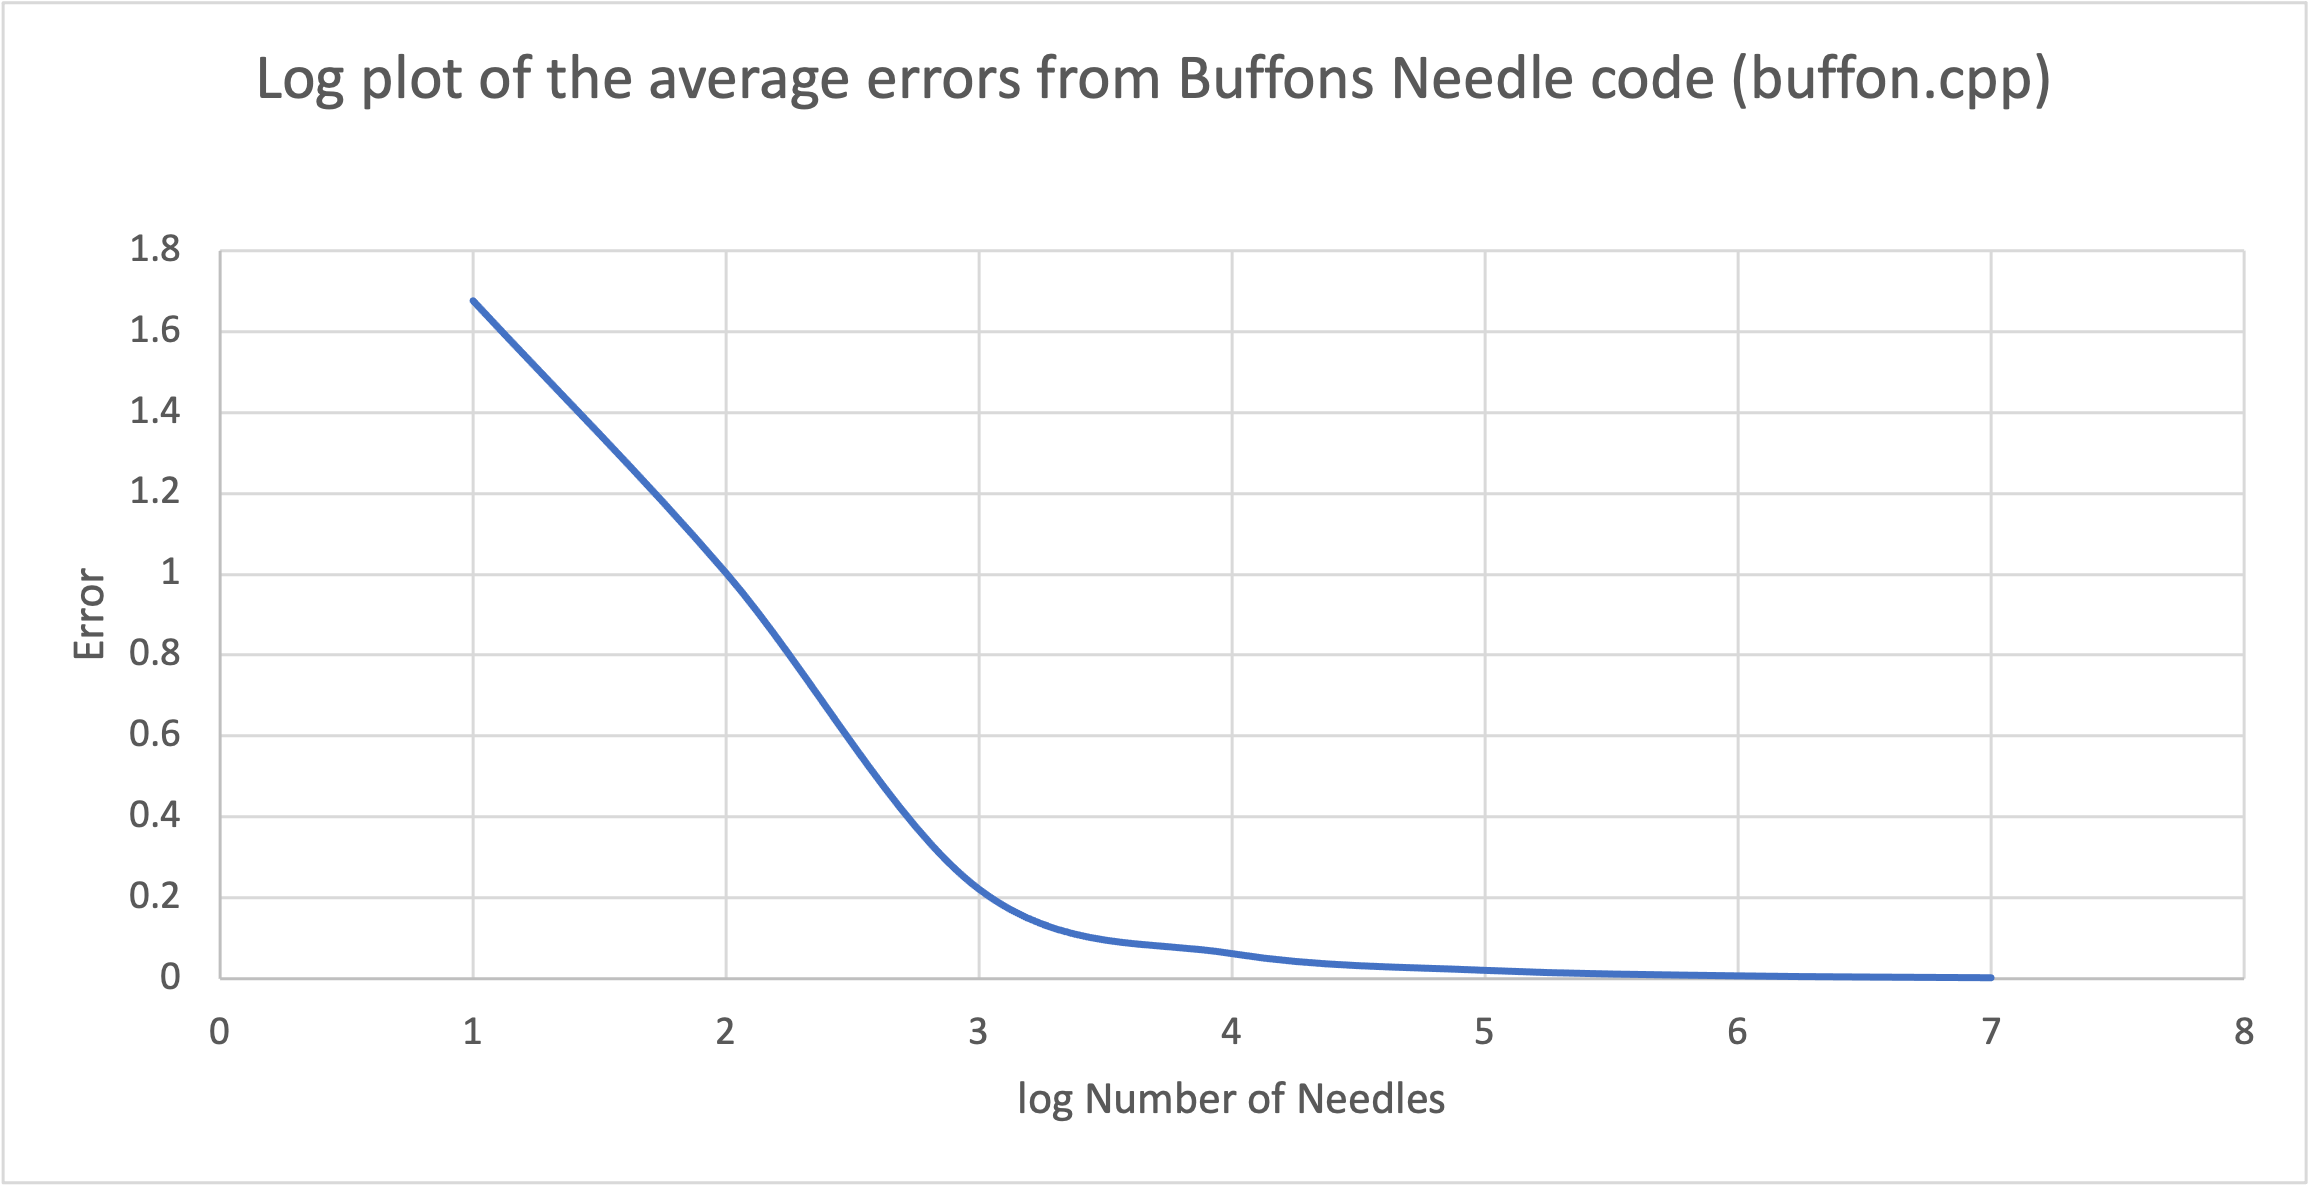
\includegraphics[width=15cm]{Picture 1.png}
    \centering
    \caption{Plot showing $ f_1 (x) = \frac{cos(x) -1}{x^2} $ as well as its taylor series approximation. As you can see the blue line has errors around the 0 point, whereas the orange line evaluate it correctly}
\end{figure}

\begin{figure}[h]
    
    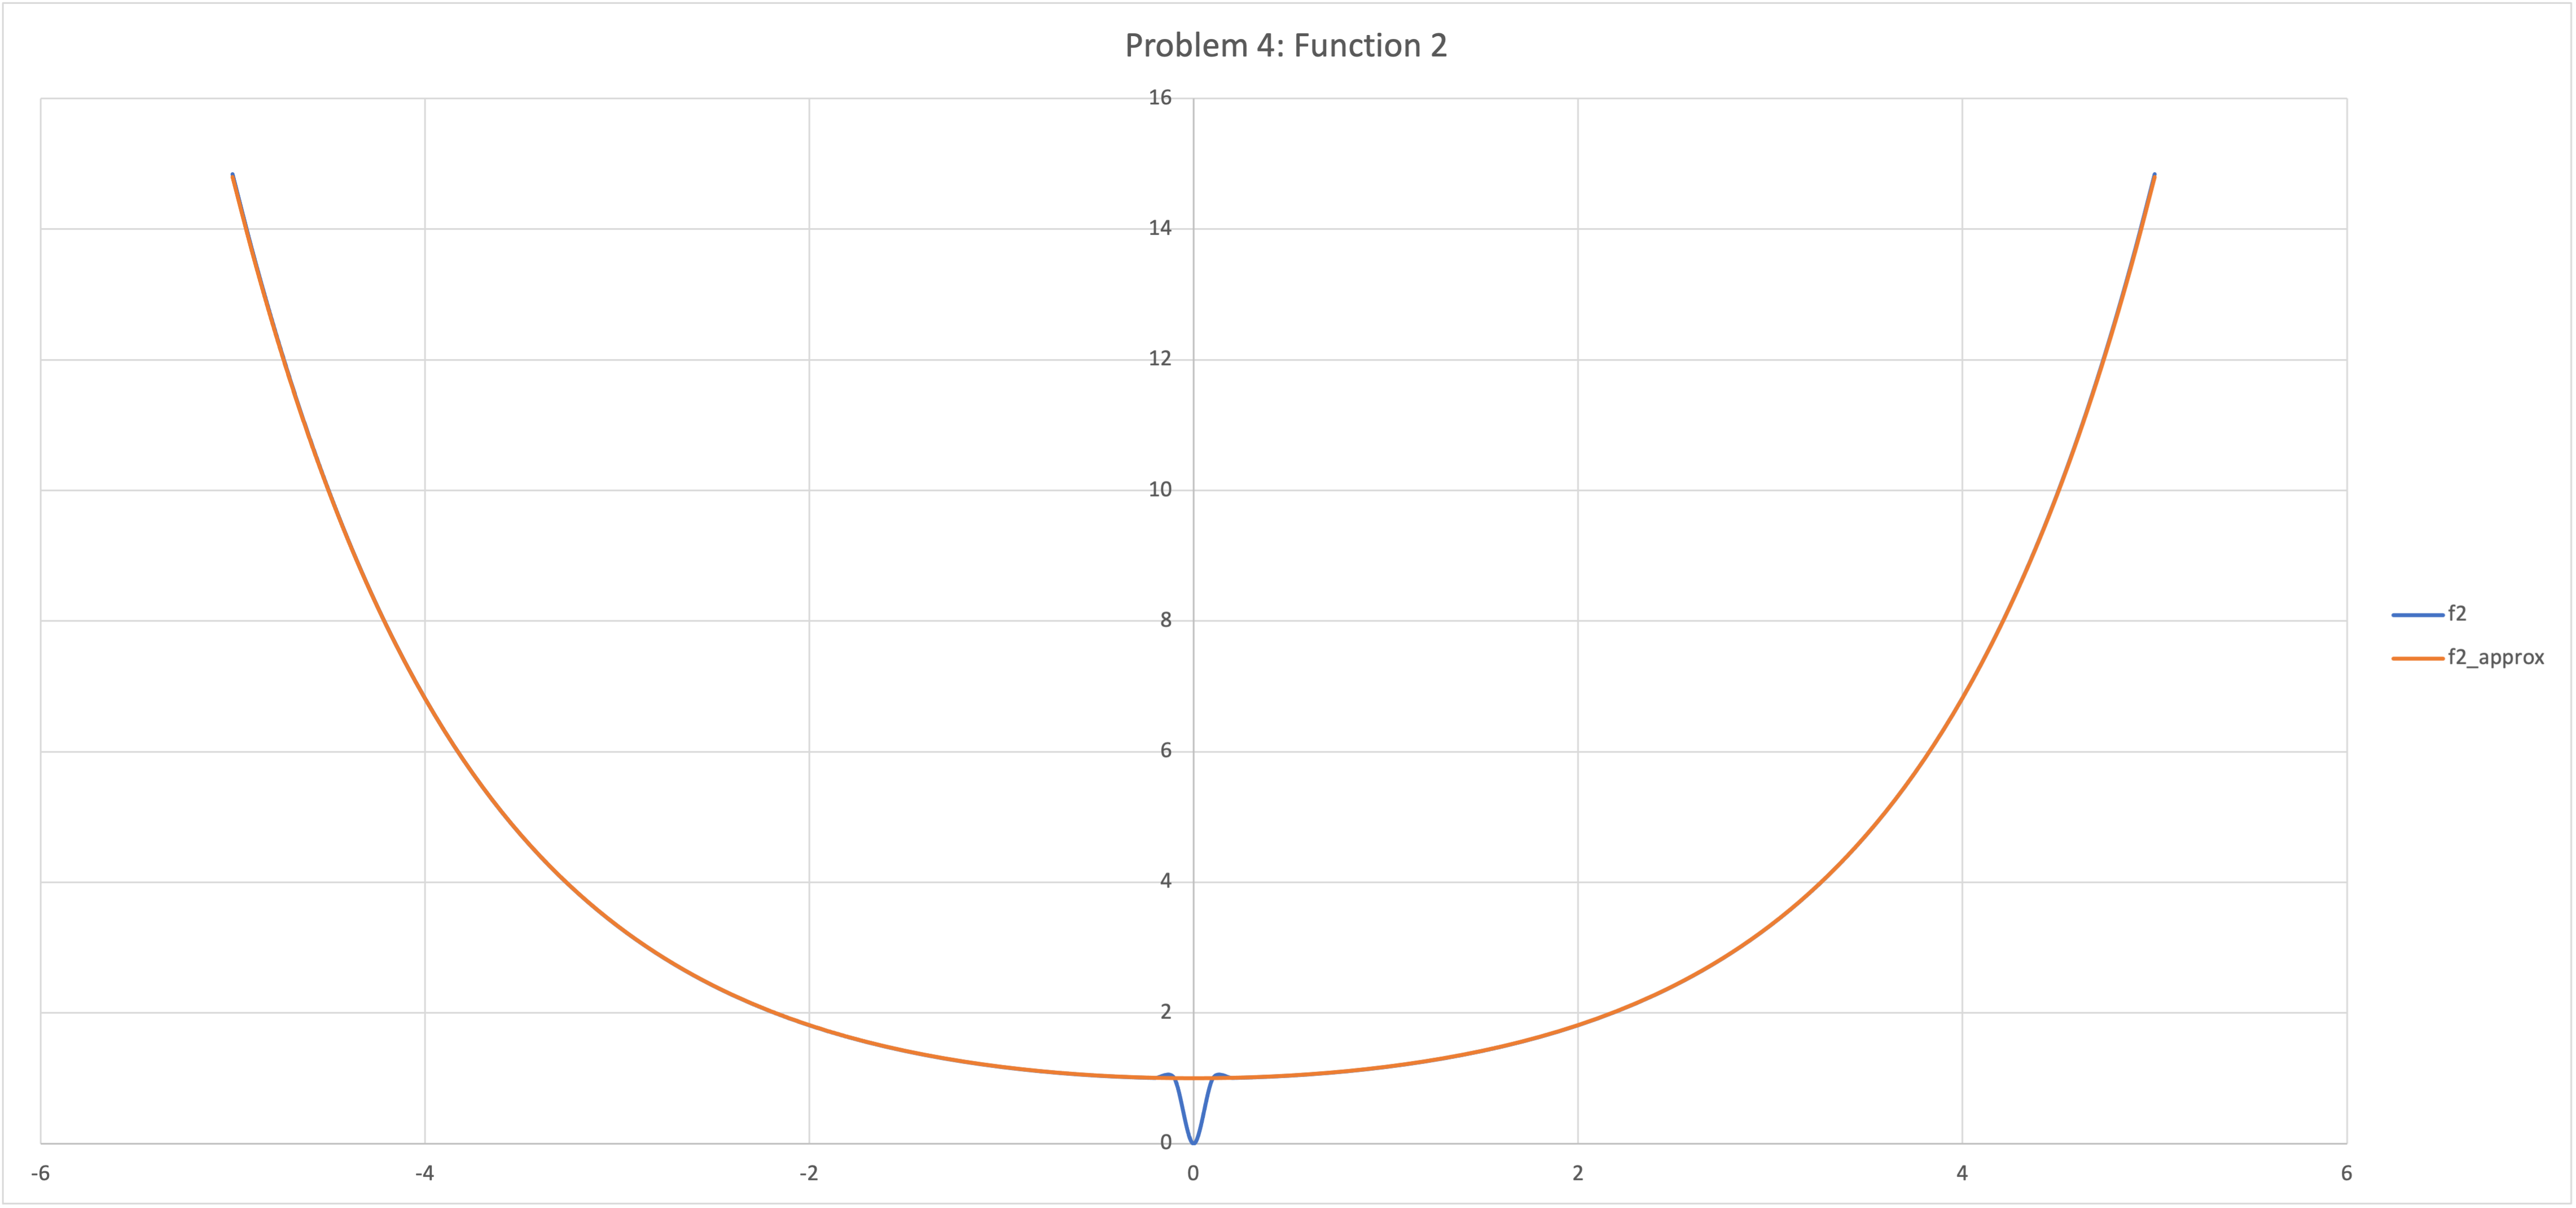
\includegraphics[width=15cm]{Picture 2.png}
    \centering
    \caption{Plot showing $ f_2 (x) = \frac{e^x - e^{-x} }{2x} $ as well as its taylor series approximation. As you can see the blue line has errors around the 0 point, whereas the orange line evaluate it correctly}

\end{figure}

\subsection*{Results}
For $x=0.00000001$
$$ f_1 (x) = 0; f_2 (x) = 1 $$
Part C:
$$ f_1(x) \approx -0.5 $$
$$ f_2(x) \approx 1 $$ 



\end{document}


